\documentclass[Ex4_Zusammenfassung.tex]{subfiles}

\begin{document}
\section{Kernspaltung}
\textbf{von \mitsch und \soeren} \newline 
Kernspaltung ist ein Prozess, bei dem en Atomkern unter Energiefreisetzung in zwei oder mehrere Kerne zerlegt wird.
\subsection{Spontane Spaltung}
Ist die Spaltung ohne äußere Energiezufuhr. \\
Bei der Spaltung müssen  die abgespaltenen Teilchen eine Potentialbarriere überwinden, den sog. Coulomb-Wall.
Wir betrachten nun die Potentialbarrieren für zwei verschiedene Arten der Spaltung.
\begin{itemize}
\item Spaltung in zwei gleich große Teile (Fission): 
		\begin{equation}
		V_{cb}^f = \frac{1.44 MeV \ fm}{r} \cdot \frac{Z}{2}^2
		\end{equation}
\item $\alpha$-Zerfall: 
		\begin{equation}
		V_{cb}^{\alpha} = \frac{1.44 MeV \ fm}{r} \cdot \underbrace{2 \ (Z-2)}_{\approx 2 \cdot Z}
		\end{equation}
\end{itemize}
Daraus erschließt man, dass i.A. die Spaltung viel unwahrscheinlicher ist, als der $\alpha$-Zerfall, da für die Tunnelwahrscheinlichkeit gilt $T \propto e^{-V}$ \\ 

Bei der Spaltung wird die annähernd kugelsymmetrische Verteilung der Nukleonen deformiert (Abb.11.6)
\begin{figure}[H]
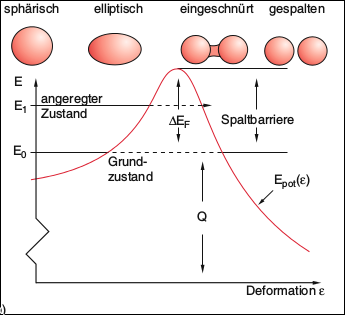
\includegraphics[scale=0.7]{Kernspaltung.png}
\caption{Schematischer Verlauf der pot. Energie bei Kernspaltung}
\end{figure}
Dabei steigt die Oberflächenspannung (Oberfläche wird stärker außeinandergezogen) 
\begin{equation}
E_{\epsilon}^S = E_0^S + \Delta E_{\epsilon}^S
\end{equation}
während die Coulomb-Energie abnimmt (Ladungsträger werden weiter außeinandergebracht, abstoßende Wirkung wird also kleiner)
\begin{equation}
E_{\epsilon}^C = E_0^C - \Delta E_{\epsilon}^C
\end{equation}
Eine spontane Spaltung tritt auf, wenn $\Delta E_{\epsilon}^C \geq \Delta E_{\epsilon}^S$, also die Gesamtenergie bei Deformation abnimmt. Dies ist der Fall, wenn $\nicefrac{Z^2}{A} \geq 51$. Bei knapp kleineren Z  ist durch Tunneleffekt noch eine spontane Spaltung möglich. Für kleinere Werte Werte von Z nimmt die Spaltung stark ab. 
\begin{figure}[H]
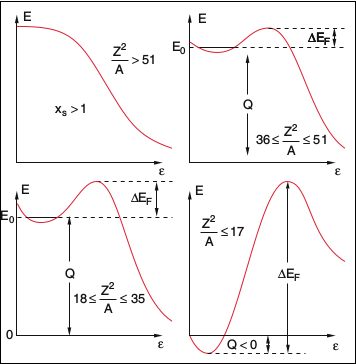
\includegraphics[scale=0.8]{Kernspaltung_Abnahme.png}
\caption{Potentialschwelle der Kernspaltung für verschiedene Werte des Verhältnisses $\frac{Z^2}{A}$}
\end{figure}
Da das Potential für große $\frac{Z^2}{A}$ stets monoton abfällt ist die Spaltung deterministisch und wird auf jeden Fall eintreten. Für kleinere $\frac{Z^2}{A}$ gibt es einen ansteigenden Bereich indem die Spaltung propabilistisch möglich ist durch den Tunneleffekt. Im abfallenden Bereich ist sie stets deterministisch. Je kleiner $\frac{Z^2}{A}$ wird, desto weiter verschiebt sich der Peak in positive $\epsilon$-Richtung, und der deterministische Bereich wird immer kleiner, wobei der propabilistische Bereich zunimmt. Wir sehen außerdem, dass die Potentialschwelle $\Delta E_F$ (Höhe des Peaks) mit abnehmendem $\nicefrac{Z^2}{A}$ größer wird. 

\subsection{Stoßinduzierte Spaltung}
Diese Spaltung passiert, wenn genug Energie aufgebracht wird, um die Oberflächenspannung zu überwinden (bei $\nicefrac{Z^2}{A} < 51$). \\ \newline
\textbf{Beispiel: Uran $^{235} U$} \newline
Uran könnte z.B durch Neutronenbeschuss zur Kernspaltung induziert werden. Dies passiert für $^{235} U$ am effektivsten wenn thermische Neutronen zum Beschuss verwendet werden (d.h $E_{Neutronen} \approx \frac{1}{40}$ eV [$k_B  T$ bei Zimmertemperatur] ) \newline
Im Allgemeinen sind die Zerfallsprodukte nicht symmetrisch. Die Töchter sind oft angeregt (zerfallen durch $\beta^-$ oder $\gamma$-Zerfall) und direkt erzeugte Neutronen. Wir betrachten dazu ein Beispiel:
\begin{equation}
^ {235} U + n \rightarrow ^{236} U ^*  \rightarrow ^{96}_{36} Kr + ^{138}_{56} Ba + 2n + \gamma
\end{equation}
Pro Spaltkern werden im Mittel 200-250 MeV frei.
\begin{itemize}
\item 83 \% davon gehen in die kinetische Energie der Fragmente
\item 2.5 \% in $E_{kin}$ von Neutronen
\item 3.5 \% in direkte $\gamma$-Strahlung 
\item 17 \% in Anregungsenergie der Spaltfragmente
\end{itemize}  
Im Mittel werden 2.5 Neutronen mit $E_k = 1-2$ MeV pro Spaltung erzeugt. Um neue Spaltungen zu induzieren, müssen diese auf thermische Energiebereiche abgebremst werden. 

\subsubsection{Begriffserklärung}
\begin{itemize}
\item Kritische Reaktion: Im Mittel wird aus den Spaltprodukten wieder 1 Kern zur Spaltung angeregt. Es entsteht eine Reaktionskette mit konstanter Rate. 
\item Superkritsche Reaktion: Mehrere induzierte Spaltungen pro Spaltprodukte. Es entsteht eine ansteigende Reaktionsrate. 
\item Subkritische Reaktion: Im Mittel wird aus den Spaltprodukten weniger als 1 Kern zur Spaltung angeregt. Die Reaktionsrate stirbt mit der Zeit aus. 
\end{itemize}

\subsubsection{Technische Punkte}
\begin{itemize}
\item Die induzierten Neutronen müssen andere Kerne treffen. Dafür wird ein hoher Dichtewert und ein kleiner $\nicefrac{Oberflaeche}{Volumen}$-Wert benötigt.
\item Neutronen müssen abgebremst werden. Es werden dafür leichtes und schweres Wasser oder Graphit benutzt. (Moderator)
\item Die Reaktion muss kontrollierbar sein. es werden Absorberstäbe aus Cadmium oder Bor für den Neutroneneinfang verwendet. 
\end{itemize}
Natürliches Uran besteht zu 99.3 \% aus $^{238} U$ und zu 0.7 \% aus $^{235} U $. Ersteres produziert keine Spaltungskette, da die Neutronen zu langsam sind um neue Spaltungen von $^{238} U$ zu induzieren. Zusätzlich fängt $^{238} U$ die von $^{235} U $ durch Spaltung erzeugten Neutronen, ohne aber sich zu spalten. Daraus folgt, dass Uran bis 3 \% von $ ^{235} U$ eingereicht werden muss, sodass eine Kettenreaktion auftreten kann.

\end{document}